\documentclass[10pt]{article}
\usepackage[margin=1in]{geometry} 
\usepackage{enumerate, xfrac, color, graphicx}
\usepackage{amsmath,amsthm,amssymb,amsfonts,mathabx}
\usepackage{booktabs}
\usepackage{caption}
\usepackage{algorithm}
\usepackage{algpseudocode}
\usepackage{pifont}
\usepackage{listings, courier}
\graphicspath{{/Users/mfzhao/Dropbox/}}
\newcommand{\N}{\mathbb{N}}
\newcommand{\Z}{\mathbb{Z}}
\lstset{breaklines=true, basicstyle=\small\ttfamily, language=R, backgroundcolor=\color{highlight}, stepnumber=5}

\definecolor{highlight}{RGB}{248,248,248}

\begin{document}
	\title{6.867 Problem Set 1}
	\date{October 1, 2015}
	\maketitle
	
\subsubsection*{Problem 1}

We implemented gradient descent in Python using an algorithm similar to the pseudocode below. The function is written in such a way that it can accept arbitrary scalar functions $f$ and gradients, $\nabla f(x)$, where $f(x)$ here is a function of an arbitrary number of parameters, $n$, and return $\min{f(x)}$.

\begin{algorithm}
\caption{Gradient Descent}
\label{GradDescent}
\begin{algorithmic}[1]
\Procedure{Gradient Descent}{}
\State Specify initial guess, step size, and convergence criteria
\State Set current guess equal to initial guess
\While{Distance between last guess and current guess location is greater than convergence criteria}
\State Calculate function at current location
\State Calculate the gradient of function at current location
\State Updated guess = take a step from current guess in direction of gradient proportional to step size
\State Calculate distance between updated guess and current guess
\State Set current guess equal to updated guess
\EndWhile{}
\EndProcedure
\end{algorithmic}
\end{algorithm}

In order to understand the effect of various hyperparameters (our initial guess, the step size, and the convergence criteria) of the algorithm, we compared the results of our gradient descent routine given a number of different parameter combinations for two different functions: $f(x) = \sum_i^n x_i^2$ and $f(x) = \sum_i^n x_i^{\frac{2}{100}} + \cos(x)$. The first of these is a convex function, whereas the second is quite non-convex, with many local minima. The results of our gradient descent algorithm for numerous values are found below.

We find that, in general, the convex function is much better behaved. Regardless of our initial guess or our learning rate, the algorithm converges to a guess in fewer than 1,000 steps, and these guess are consistently close to $x = (0,0,0,0)$, the ``true" value. The final guess' distance from the true value of $x$ is primarily a function of the convergence criteria, which makes sense - the less picky we are with our convergence criteria, the further from the true value of $x$ our final guess will be.

The non-convex, on the other hand, is much more sensitive to the hyperparameters we specify. The most notable departure from the convex function is the influence of our initial guess. It is much easier for the gradient descent algorithm to get trapped in local minima, and this is clearly illustrated in our results. While this is the most obvious difference, note that changes in both the learning rate and the convergence criteria also lead to non-trivially different guesses for $\min{f(x)}$.

Unfortunately, it might not always be convenient to specify the gradient of our scalar function, $f(x)$, explicitly. This might be because it is complicated to compute, or because no closed form solution exists. In order to get around this issue, we can approximate the gradient of the function using central differences. We approximate the $i$th element of the gradient, $\nabla_i$, as

\begin{equation}
\nabla_i \approx \frac{f(x_i+h) - f(x_i-h)}{2h}
\end{equation} 

\noindent where $h$ is some small constant (we use $h = .001$).

We see that the performance in the calculation of the gradient is identical between the analytical approach and the central difference approach. That's great! Now let's see how our gradient descent algorithm compares to two other algorithms - Broyden?Fletcher?Goldfarb?Shanno (BFGS) and Conjugate Gradient (CG). We compare both the number of iterations and function evaluations. We'll consider our algorithm in two forms - one where we pass in an explicit gradient function, and another where we estimate the gradient using the central difference method. All benchmarking is done with the same starting point: [5, -3, 7, 8]. $f_1(x) =  \sum_i^n x_i^2$ and $f_2(x) = \sum_i^n x_i^{\frac{2}{100}} + \cos(x)$. We see that when passed an analytical solution for $\nabla f(x)$, our algorithm requires about as many function calls, although many more iterations than both BFGS and CG. Given we do not have an analytical expression for $\nabla f(x)$, however, our algorithm requires many more iterations and function calls.

\begin{table}
\captionof{table}{Performance of gradient descent given various algorithm hyperparameters} 
\begin{tabular}{llllll}
\toprule
{} &                        $Guess_{i}$ &      $R_{learn}$ &   Thresh. &    $Guess_{f}$ ($f(x) = \sum_i^n x_i^2$) & $Guess_{f}$ ($f(x) = \sum_i^n x_i^{\frac{2}{100}} + \cos(x)$) \\
\midrule
&    [5.0, -3.0, 7.0, 8.0] &    0.3 &    0.1 &   [0.020, -0.012, 0.029, 0.033] &    [6.150, -0.314, 6.165, 6.176] \\
&    [5.0, -3.0, 7.0, 8.0] &    0.3 &  0.001 &   [0.001, -0.001, 0.002, 0.002] &    [6.159, -0.025, 6.160, 6.161] \\
&    [5.0, -3.0, 7.0, 8.0] &    0.3 &  1e-05 &   [0.000, -0.000, 0.000, 0.000] &    [6.160, -0.003, 6.160, 6.160] \\
&    [5.0, -3.0, 7.0, 8.0] &  0.003 &    0.1 &   [1.172, -0.703, 1.641, 1.876] &    [5.005, -2.999, 6.995, 7.993] \\
&    [5.0, -3.0, 7.0, 8.0] &  0.003 &  0.001 &   [0.118, -0.071, 0.165, 0.188] &    [6.092, -0.932, 6.200, 6.267] \\
&    [5.0, -3.0, 7.0, 8.0] &  0.003 &  1e-05 &   [0.012, -0.007, 0.017, 0.019] &    [6.092, -0.932, 6.200, 6.267] \\
 &  [-10.0, 4.0, 1.0, -5.0] &    0.3 &    0.1 &  [-0.041, 0.016, 0.004, -0.020] &  [-12.059, 6.070, 0.014, -6.139] \\
&  [-10.0, 4.0, 1.0, -5.0] &    0.3 &  0.001 &  [-0.003, 0.001, 0.000, -0.001] &  [-12.294, 6.152, 0.001, -6.158] \\
 &  [-10.0, 4.0, 1.0, -5.0] &    0.3 &  1e-05 &  [-0.000, 0.000, 0.000, -0.000] &  [-12.315, 6.159, 0.000, -6.159] \\
 &  [-10.0, 4.0, 1.0, -5.0] &  0.003 &    0.1 &  [-2.388, 0.955, 0.239, -1.194] &  [-10.002, 4.004, 0.995, -5.005] \\
 &  [-10.0, 4.0, 1.0, -5.0] &  0.003 &  0.001 &  [-0.240, 0.096, 0.024, -0.120] &  [-11.748, 5.885, 0.063, -6.076] \\
 &  [-10.0, 4.0, 1.0, -5.0] &  0.003 &  1e-05 &  [-0.024, 0.010, 0.002, -0.012] &  [-11.848, 5.938, 0.051, -6.092] \\
 &   [1.0, -1.0, -3.0, 2.0] &    0.3 &    0.1 &  [0.010, -0.010, -0.031, 0.020] &   [0.007, -0.007, -0.314, 0.024] \\
 &   [1.0, -1.0, -3.0, 2.0] &    0.3 &  0.001 &  [0.001, -0.001, -0.002, 0.001] &   [0.001, -0.001, -0.025, 0.002] \\
 &   [1.0, -1.0, -3.0, 2.0] &    0.3 &  1e-05 &  [0.000, -0.000, -0.000, 0.000] &   [0.000, -0.000, -0.003, 0.000] \\
 &   [1.0, -1.0, -3.0, 2.0] &  0.003 &    0.1 &  [0.736, -0.736, -2.207, 1.471] &   [0.995, -0.995, -2.999, 1.994] \\
 &   [1.0, -1.0, -3.0, 2.0] &  0.003 &  0.001 &  [0.073, -0.073, -0.220, 0.147] &   [0.051, -0.051, -0.932, 0.143] \\
 &   [1.0, -1.0, -3.0, 2.0] &  0.003 &  1e-05 &  [0.007, -0.007, -0.022, 0.015] &   [0.051, -0.051, -0.932, 0.143] \\
\bottomrule
\end{tabular}
\end{table}

\begin{table}
\captionof{table}{Performance in gradient calculation for analytical and central difference approaches} 
\begin{tabular}{llllll}
\toprule
{} &   $x_{i}$  &  function &   $\nabla_{analytical}$  & $\nabla_{approximate}$ \\
\midrule
&    [5.0, -3.0, 7.0, 8.0] & $f(x) = \sum_i^n x_i^2$ &  [ 10.  -6.  14.  16.] & [ 10.  -6.  14.  16.]\\
&    [5.0, -3.0, 7.0, 8.0] & $f(x) = \sum_i^n x_i^{\frac{2}{100}} + \cos(x)$ & [-0.8589 -0.2011  0.797   1.1494] &[-0.8589 -0.2011  0.797   1.1494] \\
&    [-10.   4.   1.  -5.] & $f(x) = \sum_i^n x_i^2$ &   [-20.   8.   2. -10.] &  [-20.   8.   2. -10.]\\
&    [-10.   4.   1.  -5.] & $f(x) = \sum_i^n x_i^{\frac{2}{100}} + \cos(x)$ &[ 0.344  -0.6768  0.8615  0.8589]&[ 0.344  -0.6768  0.8615  0.8589] \\
&    [ 1. -1. -3.  2.] & $f(x) = \sum_i^n x_i^2$ &  [ 10.  -6.  14.  16.] & [ 10.  -6.  14.  16.]\\
&    [ 1. -1. -3.  2.] & $f(x) = \sum_i^n x_i^{\frac{2}{100}} + \cos(x)$ & [ 0.8615 -0.8615 -0.2011  0.9493] & [ 0.8615 -0.8615 -0.2011  0.9493] \\
\bottomrule
\end{tabular}
\end{table}

\begin{table}
\captionof{table}{Performance of authors' gradient descent algorithm compared to BFGS and CG}
\begin{tabular}{llllll}
\toprule
{} & algorithm & $f_1(x)$ function calls & $f_1(x)$ iterations &  $f_2(x)$ function calls &  $f_2(x)$ iterations \\
\midrule
  & BFGS & 24 & 2 & 78 & 10 \\
  & CG & 30 & 2 & 78 & 6 \\
  & Gradient Descent (analytical) & 20 & 10 & 48 & 24 \\ 
  & Gradient Descent (approximate) & 100 & 10 & 240 & 24 \\
\bottomrule
\end{tabular}
\end{table}

\subsubsection*{Problem 2}

\subsubsection*{Problem 3}

To begin problem 3, we implemented the closed form solution of Ridge Regression in Python, making use of Scipy and Numpy. Note that if you want to test cases where the number of features is greater than the number of data points (something that a well-trained teacher of machine should be skeptical to do), it is useful to calculate the inverse of a matrix using the pseudo-inverse, rather than the inverse. We learned this the long way after debugging code for hours.

The closed form solution for ridge regression is given by the expression:

\begin{equation}
\hat{\theta} = (\mathbf{X}^T\mathbf{X} + \lambda \mathbf{I})^{-1}\mathbf{X}^t\mathbf{y}
\end{equation}

\noindent where $\mathbf{X}$ is your matrix of features, $y$ is your array of observed values, and $\hat{\theta}$ are your estimated feature weights. $\lambda$ is a regularization parameter, which represents how much you penalize the model for having large feature weights.

Given the data in Bishop 1.4 (which can be seen below), we attempt to fit polynomials of various orders, $M$. 

\begin{center}
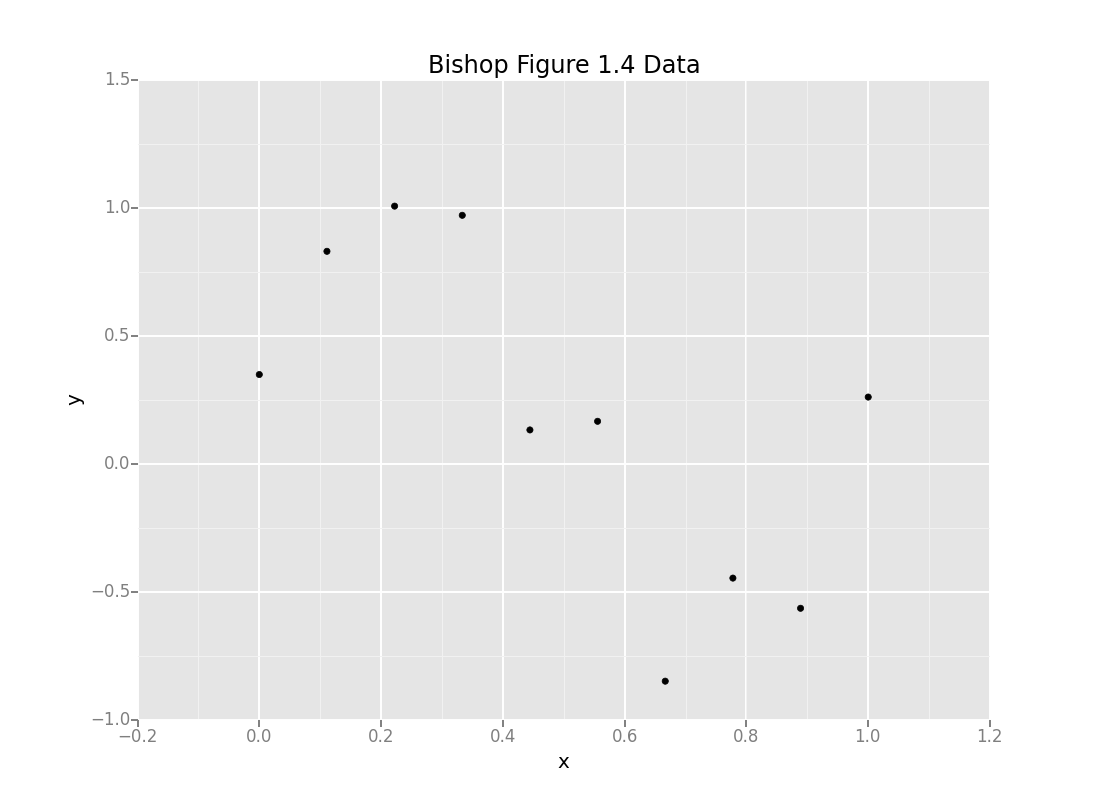
\includegraphics[scale=.3]{Bishop_14_Data.png}
\end{center}

The plot below shows the mean squared error (MSE) that our ridge regression fit gives for values of $M$ between 1 and 5, for values of $\lambda$ ranging from $10^0 -1$ to $10^2$. Note that in the case where $\lambda = 0$, we have $OLS$ regression, and as $M$ increases, the model is free to overfit our data. While the MSE here is low, if we evaluated this on a new data point, our model would likely perform very poorly. As $\lambda$ gets higher, we penalize the model for adding additional large weights to $\hat{\theta}$, but our $MSE$ stays relatively large. However, these ``large" MSE models are likely to perform better on a new data point!

\begin{center}
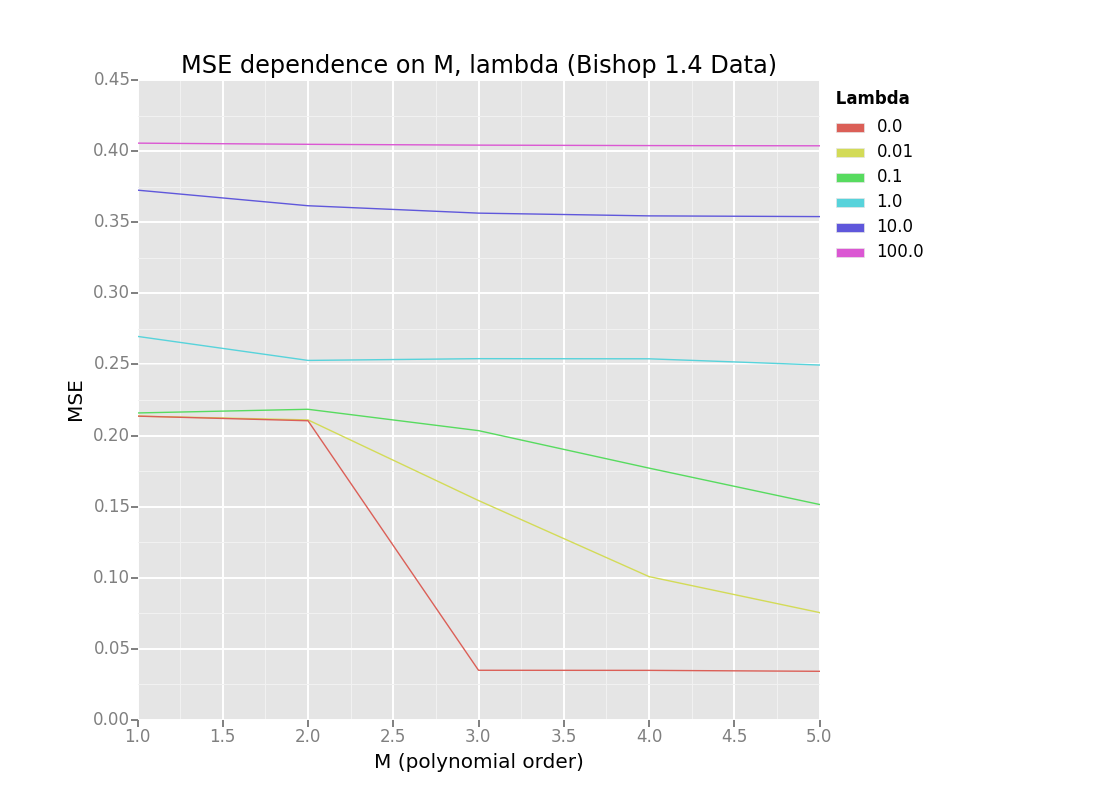
\includegraphics[scale=.4]{MSE_Lambda_Bishop.png}
\end{center}

In order to avoid overfitting, but in order to make sure that we have chosen values of $\lambda$ and $M$ (and in general, hyperparameters) that make sense, it is common to split the data into a training set and a test set. We will use the closed-form solution for ridge regression to calculate $\hat{\theta}$ on our training set. We will then use that $\hat{\theta}$ to attempt to predict values of $\mathbf{y}$ for the test data. By choosing the $\hat{\theta}$ that minimizes MSE on the test data, but is trained on the training data, we are ensuring that we have not overfit our model to the data it is trained on. As one final step in the model selection process, we can check the performance of our final $\hat{\theta}$ on a validation set, to make sure that performance is still good (and we have not overfit for performance on our test set).


\subsubsection*{Problem 4}


	
\end{document}